%!TEX program = xelatex
\documentclass[10pt, compress]{beamer}
\usetheme[titleprogressbar]{m}

\usepackage{booktabs, listings}
\usepackage[scale=2]{ccicons}
\usepackage{minted}

\usepgfplotslibrary{dateplot}

\usemintedstyle{trac}

\title{RMUAST Module 7}
\subtitle{}
\author{Christian, Vasilis, Henrik \& Asbjørn}
\institute{Group 5}

\begin{document}

\maketitle

\begin{frame}[fragile]
\frametitle{AutoQuad Log File}
UKF\_POSD
\begin{figure}
  \centering
 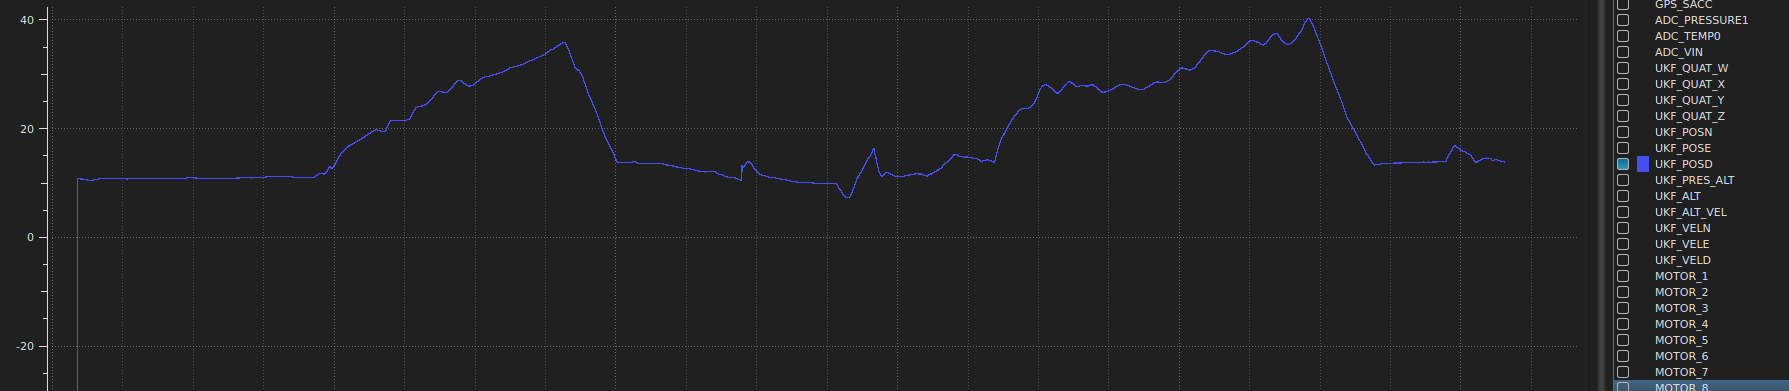
\includegraphics[width=1.1\textwidth]{Figures/2}
\end{figure}

\end{frame}

\begin{frame}[fragile]
  \frametitle{AutoQuad Log File}
  UFK\_POSN, UKF\_POSE \& UKF\_POSD
\begin{figure}
  \centering
 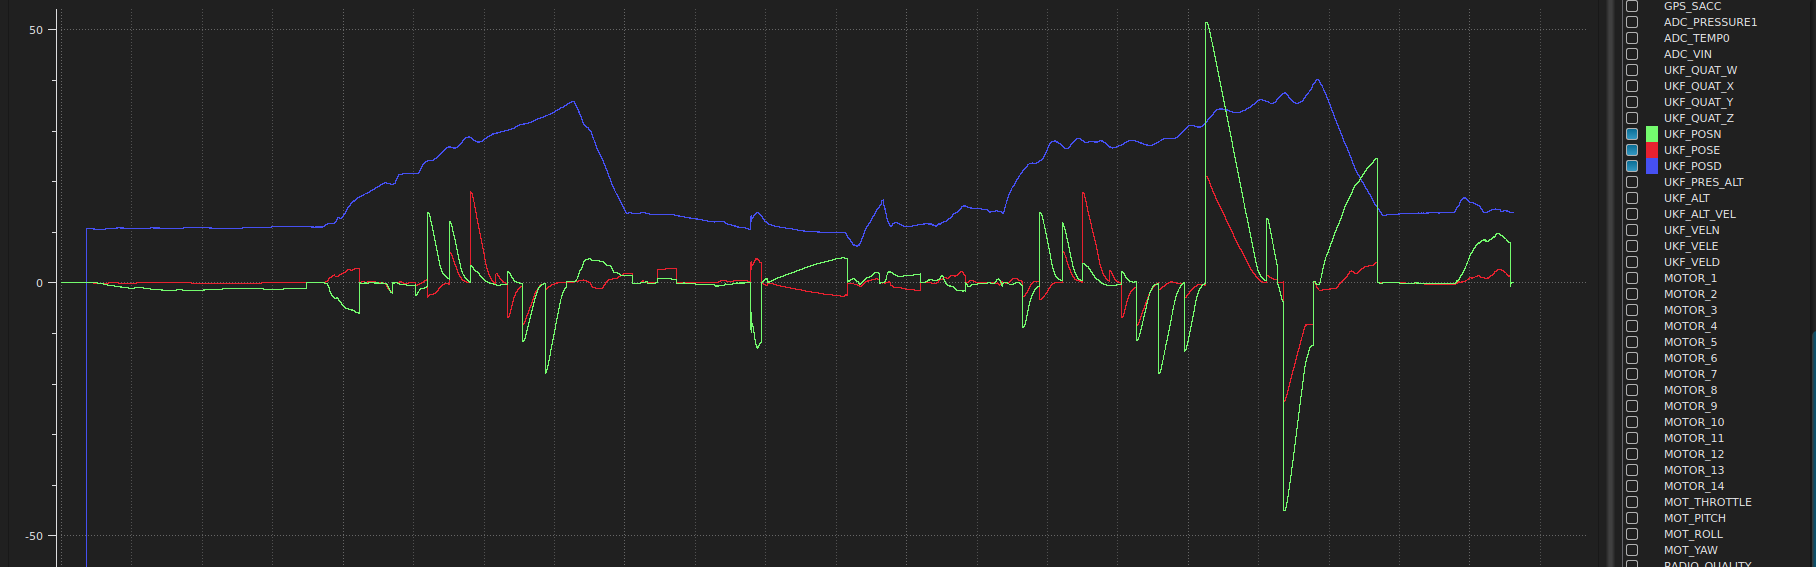
\includegraphics[width=1.1\textwidth]{Figures/1}
\end{figure}
\end{frame}


\begin{frame}[fragile]
	\frametitle{Generating Mission Route Plans}
\begin{minted}[mathescape,
%                linenos,
               numbersep=5pt,
               baselinestretch=1,
               fontsize=\footnotesize,
               gobble=2,
               frame=lines,
               framesep=2mm]{python}
   from math import hypot
        ...
        dstnc = hypot(nextLat, nextLng)
        dstnc = hypot(dstnc, nextAlt)
        # dstnc = sqrt(nextLng**2 + nextLng**2 + nextAlt**2)
        if dstnc >= threshold:
            initLat = oldLat
            initLng = oldLng
            initAlt = coords
            cpLat.append(oldLat)
            cpLng.append(oldLng)
            corAlt.append(coords)
        ...
\end{minted}
\end{frame}

\begin{frame}[fragile]
	\frametitle{Generating Mission Route Plans}
\begin{figure}
\centering
\begin{minipage}{.5\textwidth}
	\centering
	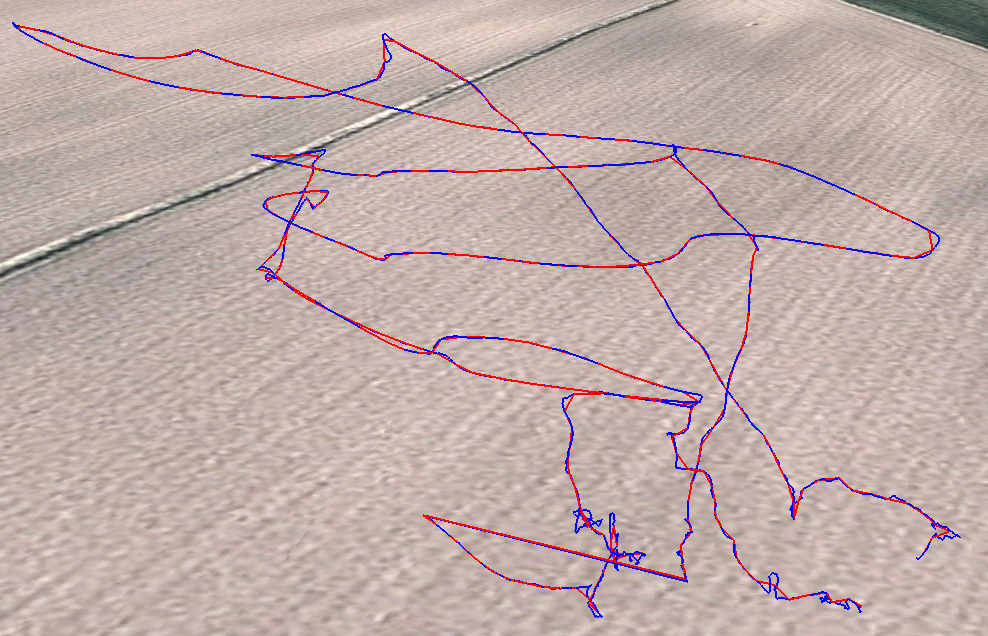
\includegraphics[width=1\linewidth]{Figures/Paths_threshold_1_w_alt}
	\caption{\textit{Threshold 1}}
	\label{fig:thresh1}
\end{minipage}%
\begin{minipage}{.5\textwidth}
	\centering
	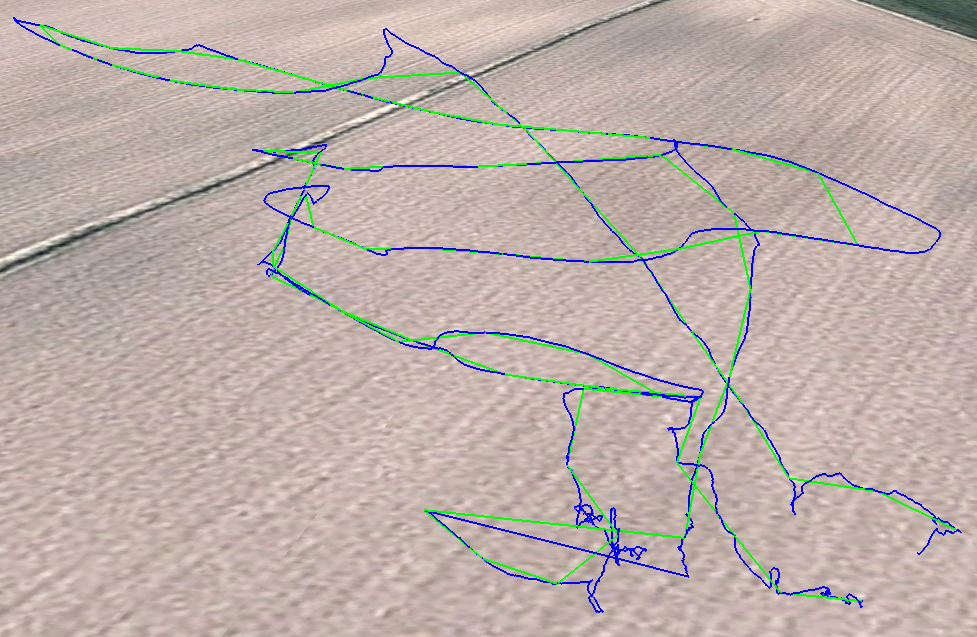
\includegraphics[width=1\linewidth]{Figures/Paths_threshold_5_w_alt}
	\caption{\textit{Threshold 5}}
	\label{fig:thresh5}
\end{minipage}
\end{figure}
\end{frame}

\begin{frame}
	\frametitle{Generating Mission Route Plans}
\begin{figure}
  \centering
 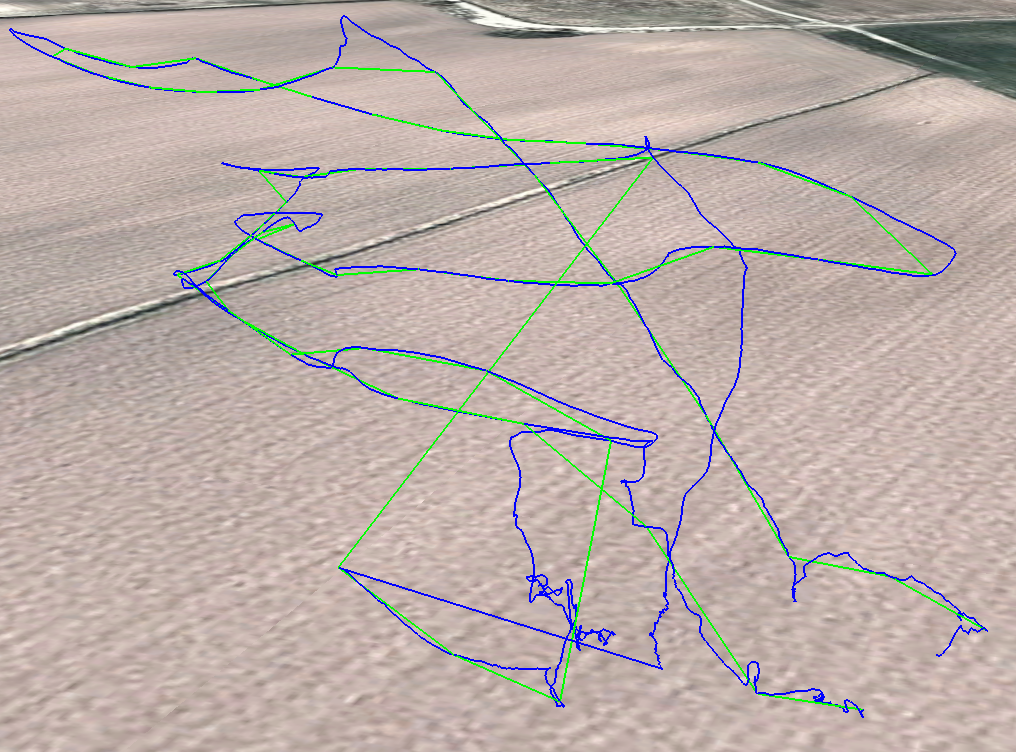
\includegraphics[width=.6\textwidth]{Figures/Paths_threshold_5}
 	\caption{\textit{Threshold 5 without taking altitude into account}}
	\label{fig:thresh5}
\end{figure}
\end{frame}

%\plain{Questions?}

\end{document}